\subsection{Mass damper spring system}

In this example we will consider the following system.

\begin{figure}[H]
	\centering
	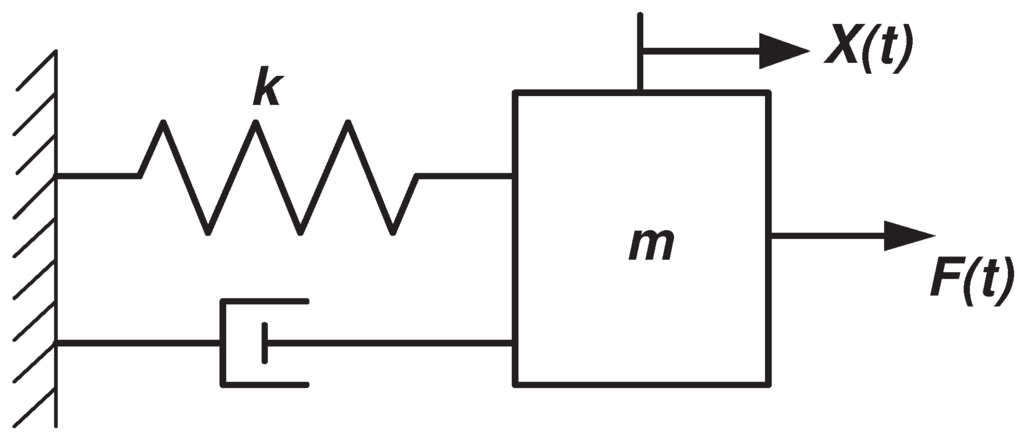
\includegraphics[scale=0.15]{Latex/image/ex-msd/msd-system.png}
	\caption{Free body diagram of the system}
	% Todo: make own image
\end{figure}

This system has the following state space representation:

\[
	\begin{bmatrix}
		\dot{x} \cr \ddot{x}
	\end{bmatrix}
	= 
	\begin{bmatrix}
		0 & 1 \cr \frac{-k}{M} & \frac{-f_v}{M}
	\end{bmatrix}
	\begin{bmatrix}
		x \cr \dot{x}
	\end{bmatrix}
	+
	\begin{bmatrix}
		0 \cr \frac{1}{M}
	\end{bmatrix}
	u
\]
\begin{lstlisting}
k = 1;
M = 1;
f = 1;
A = [0 1 ; -k/M -f/M];
B = [0 ; 1/M];
C = [1 0 ; 0 1];
D = [];
sys_mds_c = ss(A,B,C,D);
\end{lstlisting}

\subsubsection{Impulse response}
For this example we will consider data generated by the impulse response of this system.

\begin{lstlisting}
[y_impulse, t_impulse, x_impulse] = impulse(sys_mds_c);
\end{lstlisting}

\begin{figure}[H]
	\centering
	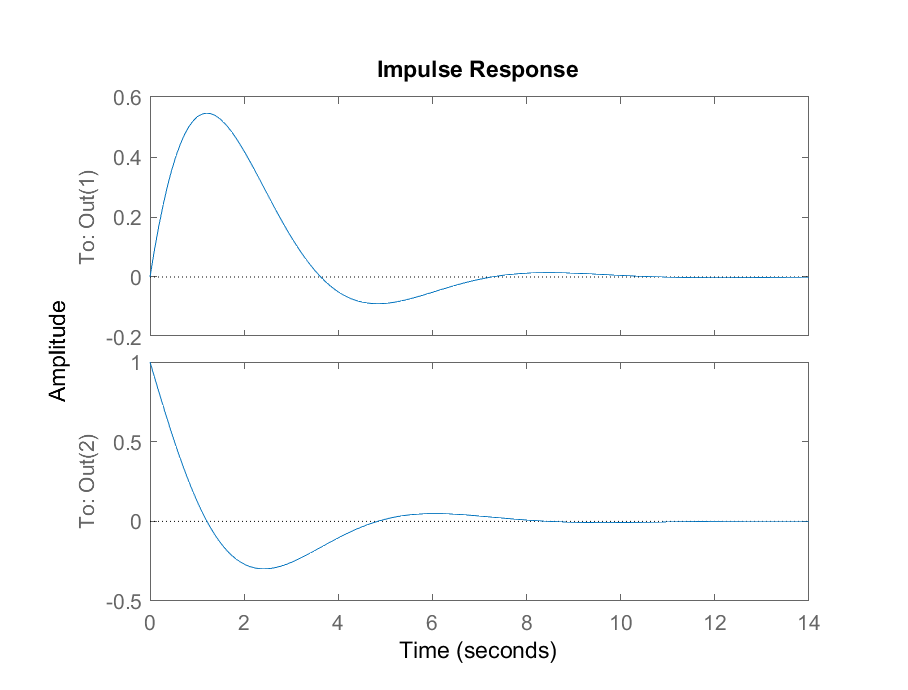
\includegraphics[width=0.5\textwidth]{Latex/image/ex-msd/impulse.eps}
	\caption{Impulse response of the mass damper spring system}
\end{figure}

\paragraph{Defining the data}
We will first consider all 150 datapoints generated by the impulse function. Since we are considering the impulse responce we have that our input is infinitly small and thus bassically non existing. Because of this we can only use the impulse respons to find the $A$ matrix of the system, since we are considering the system as if it had no input. But first we need to put the data as returned by the impulse function in the correct format.
\begin{lstlisting}
X_impulse = x_impulse.';
\end{lstlisting}

\paragraph{System identification}
We can check if the data is informative for system identification by using:
\begin{center}
	\mon{[bool, A] = isIdentifiable(X)}
\end{center}
For this to be the case we need that the data is full rank, i.e.:
\[ rank\left( \begin{bmatrix}
X_- \\ U_-
\end{bmatrix} \right) = n + m\]

Since we use the impulse function we know that $U_-$ is empty and $m$ is zero. Hence we only need to find 2 linearly independant columns in our data points. From this we can see that the use of 150 data points is a bit eccesive, thus we also consider some cases below where we reduce the amount of data points.

\begin{lstlisting}
disp("Is the data informative for system identification?");
[bool, A_impulse] = isInformIdentification(X_impulse)
\end{lstlisting}

\begin{verbatim}
Is the data informative for system identification?
bool = 
  1
A_impulse =
  0.9959    0.0879
 -0.0879    0.9080
\end{verbatim}

We will use the received A matrix to verify the data.

\subparagraph{Verifying results}
We can check the validity of the results by comparing them against the continuous time version of the system. To get the continuous time system we use the \mon{sysc = d2c(sysd)} function provided by Matlab. We can find the timestep of the data by inspecting the \mon{t\_impulse} array that was returned by the impuls function.

\begin{lstlisting}
disp("What does the obtained system look like in continuous time form?")
sys_impulse_d = ss(A_impulse, [], C, D, t_impulse(2));
sys_impulse_c = d2c(sys_impulse_d)
\end{lstlisting}

\begin{verbatim}
What does the obtained system look like in continuous time form?
sys_impulse_c =
  A = 
               x1         x2
    x1  -3.24e-15          1
    x2         -1         -1
  B = 
    Empty matrix: 2-by-0
  C = 
        x1  x2
    y1   1   0
    y2   0   1   
  D = 
    Empty matrix: 2-by-0
Continuous-time state-space model.
\end{verbatim}

As we can see, we are able to retreive the $A$ matrix using the imulse response of the system. But to retreive the $B$ matrix we need a non zero input for the system. For this we will consider the step response. But first we will look if the data is informative for stability.

\subsubsection{Stability}
We can also check if the data is informative for stability. Looking at the plot of the impulse response (or the eigenvalues of $A$), we would expect this to be the case. We can verify this by using the function:
\begin{center}
	\mon{bool = isInformStable(X)}
\end{center}

\begin{lstlisting}
disp("Is the data informative for stability?");
disp(isInformStable(X_impulse));
\end{lstlisting}

This will result in the following output:

\begin{verbatim}
Is the data informative for stability?
1
\end{verbatim}

\subsubsection{Step response}
As noted above, we will use the step response to retrieve the $A$ and $B$ matrix describing the system.

\paragraph{Defining data}
We will start by considering all 150 data points generated by the step function. We will see later on that this is excessive and that we can use less points for the same result. Since the step function is a constant unit input, we will define $U_-$ in the following way:
\begin{lstlisting}
[y_step, t_step, x_step] = step(sys_mds_c);
U_step = ones(1,149);
X_step = x_step.';
\end{lstlisting}

\begin{figure}[H]
	\centering
	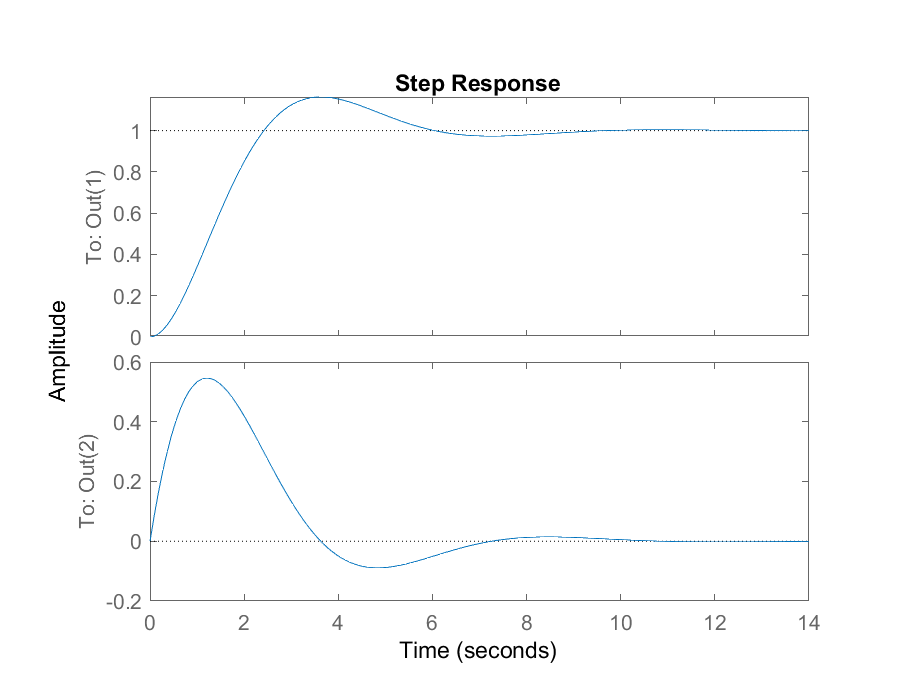
\includegraphics[width=0.5\textwidth]{Latex/image/ex-msd/step.eps}
	\caption{Step response of the mass damper spring system}
\end{figure}

\paragraph{System identification}
To see if the data is informative for system identification we will once again consider the following function:
\begin{center}
	\mon{[bool, A, B] = isIdentifiable(X, U)}
\end{center}

\begin{lstlisting}
disp("Is the data informative for system identification?");
[bool, A_step, B_step] = isInformIdentification(X_step, U_step)
\end{lstlisting}

This will result in the following output:

\begin{verbatim}
Is the data informative for system identification?
bool =
  1
A_step =
   0.9959    0.0879
  -0.0879    0.9080
B_step =
   0.0041
   0.0879
\end{verbatim}

\subparagraph{Verifying results}
We will once again check the validity of the data by first converting the system back to a continuous time system using the \mon{sysc = d2c(sysd)} function provided by Matlab, using the same timestep as the data, namely \mon{t\_step(2)}.

\begin{lstlisting}
disp("What does the obtained system look like in continuous time form?")
sys_step_d = ss(A_step, B_step, C, D, t_step(2));
sys_step_c = d2c(sys_step_d)
\end{lstlisting}

This will result in the following output:

\begin{verbatim}
What does the obtained system look like in continuous time form?
sys_step_c =
  A = 
              x1         x2
   x1  4.822e-15          1
   x2         -1         -1
  B = 
              u1
   x1  3.466e-15
   x2          1
  C = 
       x1  x2
   y1   1   0
   y2   0   1
  D = 
       u1
   y1   0
   y2   0
Continuous-time state-space model.
\end{verbatim}

As we can see we get the valid $A$ and $B$ matrix (up to working precision). Thus we can conclude that the impulse response is insufficient for finding the $B$ matrix of the system. It is however still informative for identification of the A matrix. The step response however is sufficient for finding both the $A$ and $B$ matrix of the system.

Even though we have found the system to be uniquely identifiable, we will still see if we can infer other properties from the data. We will then confirm these properties based on the true system.

\subsubsection{Controllability}
In this section we will see if the data is informative for controllability. We can check this using the function:
\begin{center}
	\mon{bool = isControllable(X)}
\end{center} 

\begin{lstlisting}
disp("The data is informative for controllability?");
disp(isInformControllable(X_step));
\end{lstlisting}

\begin{verbatim}
The data is informative for controllability?
  1
\end{verbatim}

As we can see the data is informative for controllability. We can verify this by means of the reachability matrix of the actual system.

\begin{lstlisting}
disp("The system is controllable?");
disp(rank([B A*B]) == 2);
\end{lstlisting}

\begin{verbatim}
The system is controllable?
  1
\end{verbatim}

\subsubsection{Stabilisability}
In this section we will see if the data is informative for stabilisability. We can check if the data is informative for stabilisability by using the function:
\begin{center}
	\mon{bool = isStabilisable(X)}
\end{center} 

\begin{lstlisting}
disp("The data is informative for system stabilisability?");
disp(isInformStabilisable(X_step))
\end{lstlisting}

\begin{verbatim}
The data is informative for system stabilisability?
  1
\end{verbatim}

As expected, the data is informative for stabilisability. This is what we would expect since if a system is controllable it should also be stabilisable.

\subsubsection{State feedback}
Since our system is controllable, we might want to find a state feedback controller, in this example it is unneccesary since the system is already stable, but lets assume we are not aware of this. To find a full state feedback controller we can use the function:
\begin{center}
	\mon{[bool, K, diagnostics] = StateFeedbackYalmip(X, U, tolerance, options)}
\end{center} 

\begin{lstlisting}
[bool, K, diagnostics] = StateFeedbackYalmip(X_step, U_step);
\end{lstlisting}

Since we have that the data is also informative for system identification, we can verify the result.

\begin{lstlisting}
disp("Is the data informative for state feedback?");
disp(bool);
disp("The eigenvalues of A+BK are:");
disp(eig(A_step + B_step * K));
disp("Their magnitude is:");
disp(abs(eig(A_step + B_step * K)));
\end{lstlisting}

\begin{verbatim}
Is the data informative for state feedback?
  1
The eigenvalues of A+BK are:
  0.9996 + 0.0182i
  0.9996 - 0.0182i
Their magnitude is:
  0.9998
  0.9998
\end{verbatim}

Thus the provided controller is indeed a stabilizing controller, al be it a slow one. Currently it is not possible to place the poles for the given controller.

\subsubsection{Deadbeat control}
Since our system is controllable, we might want to find a deadbeat controller. A deadbeat controller is a controller that brings the system to a stable state in 1 iterarion. This is done by finding a controller that assigns the eigenvalues of the closed loop system to zero. To do this we will use the function:
\begin{center}
	\mon{[bool, K] = isInformDeadbeatControl(X, U)}
\end{center}

\textbf{TODO: currently the \mon{isInformDeadbeatControl} function is not working properly}



\subsubsection{How much data is needed and what is the precision}
We will now look at how much data we need for system identification, for this we will check the first n entries of the step response data. We will also use these results to check the consistency of the result based on the amount of data provided.

\begin{lstlisting}
n = 149;
isIdentifiable = [];
a11 = []; a12 = []; a21 = []; a22 = [];
b1  = []; b2  = [];
for idx = 1:n
    [bool,A_temp,B_temp] = isInformIdentification(X_step(:,1:idx+1), U_step(:,1:idx));
    if bool
        isIdentifiable = [isIdentifiable idx];
        a11 = [a11 A_tmp(1,1)];
        a12 = [a12 A_tmp(1,2)];
        a21 = [a21 A_tmp(2,1)];
        a22 = [a22 A_tmp(2,2)];
        b1  = [b1  B_tmp(1)];
        b2  = [b2  B_tmp(2)];
    end
end
\end{lstlisting}

From this we can inspect the \mon{isIdentifiable} array and see for how many data points the data is informative for system identification. As we noted earlier, we only needed 3 linearly independant collumns, which where the 1st, 2nd and 3rd collumn in this case.

\begin{lstlisting}
disp("How many data points are needed for system identification?:")
valid
\end{lstlisting}

\begin{verbatim}
How many data points are needed for system identification?:
isIdentifiable =
   3   4   5   6   7   8   9  10  11 ...
\end{verbatim}

We can also verify that the received $A$ matrix is consistent. To do this we will normilize out \mon{a11}, \mon{a12}, \mon{...}, \mon{b2} with the actual  and  matrix and plot the error.

\begin{lstlisting}
sys_mds_d = c2d(sys_mds_c, t_impulse(2));
x = isIdentifiable;
plot(x, a11 - sys_mds_d.A(1,1), 'DisplayName', 'a11');
hold on
plot(x, a12 - sys_mds_d.A(1,2), 'DisplayName', 'a12');
plot(x, a21 - sys_mds_d.A(2,1), 'DisplayName', 'a21');
plot(x, a22 - sys_mds_d.A(2,2), 'DisplayName', 'a22');
plot(x, b1  - sys_mds_d.B(1),   'DisplayName', 'b1');
plot(x, b2  - sys_mds_d.B(2),   'DisplayName', 'b2');
title("Error in received A and B matrix");
xlabel("Number of datapoints used");
ylabel("Normilised error");
%legend;
hold off
\end{lstlisting}

\textbf{TODO: plot legend is not working correctly (.eps was also not working correctly)}

\begin{figure}[H]
	\centering
	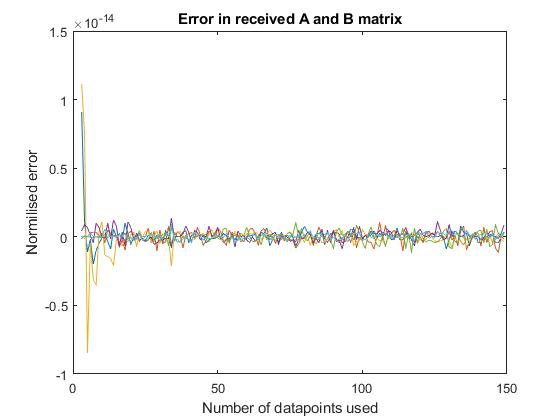
\includegraphics[width=0.5\textwidth]{Latex/image/ex-msd/lessData.jpg}
	\caption{Element-wise error for the retreived system}
\end{figure}

As we can see the received $A$ and $B$ matrix are consistent up to machine precision.

\subsubsection{What is the impact of sampling moment?}
We will now consider what happence when we skip the first few entries. We want that the result stays consistent independant of when we sample the system. Thus we use the following code to generate $A$ and $B$ using increasingly more data. 

\begin{lstlisting}
n = 100;
isIdentifiable = [];
a11 = []; a12 = []; a21 = []; a22 = [];
b1  = []; b2  = [];
for idx = 1:n
    [bool,A_tmp,B_tmp] = isInformIdentification(X_step(:,idx:end), U_step(:,idx:end));
    if bool
        isIdentifiable = [isIdentifiable idx];
        a11 = [a11 A_tmp(1,1)];
        a12 = [a12 A_tmp(1,2)];
        a21 = [a21 A_tmp(2,1)];
        a22 = [a22 A_tmp(2,2)];
        b1  = [b1  B_tmp(1)];
        b2  = [b2  B_tmp(2)];
    end
end
\end{lstlisting}

We can now normalize and plot the data to see what happens with the error.

\begin{lstlisting}
x = isIdentifiable;
plot(x, a11 - sys_mds_d.A(1,1), 'DisplayName', 'a11');
hold on
plot(x, a12 - sys_mds_d.A(1,2), 'DisplayName', 'a12');
plot(x, a21 - sys_mds_d.A(2,1), 'DisplayName', 'a21');
plot(x, a22 - sys_mds_d.A(2,2), 'DisplayName', 'a22');
plot(x, b1  - sys_mds_d.B(1),   'DisplayName', 'b1');
plot(x, b2  - sys_mds_d.B(2),   'DisplayName', 'b2');
title(gca,"Max error between found A and the actual A")
xlabel('Starting index of data array')
ylabel('Biggest element-wise error')
%legend;
hold off
\end{lstlisting}

\textbf{TODO: plot legend is not working correctly (.eps was also not working correctly)}

\begin{figure}[H]
	\centering
	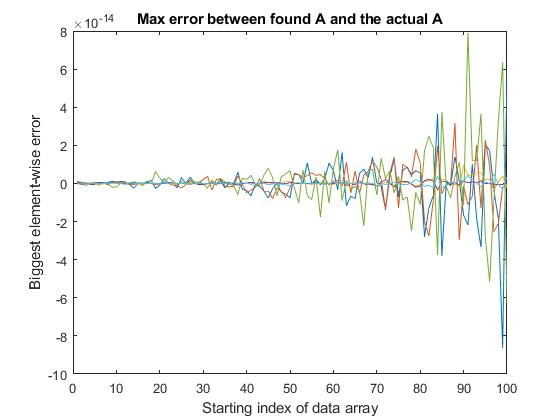
\includegraphics[width=0.5\textwidth]{Latex/image/ex-msd/startingPos.jpg}
	\caption{Element-wise error for the retreived system}
\end{figure}

As we can see the error is relativly small but increasing. This is due to noice introduced by floating point inaccuracies when the system is almost in a stable state.




















